\documentclass{article}
\usepackage{graphicx}
\usepackage{geometry}
\usepackage{tikz-cd}
\usepackage{amsmath}

\geometry{a4paper,scale=0.8}

\begin{document}
\title{Lab 1: Modeling Packet Losses}
\author{Zhipeng Ye}
\maketitle
    \section{Hidden Markov Model}
    Gilbert-Elliott Model is packet loss model which is based on two-state Hidden Markov Model.
    In other words, Gilbert-Elliott Model is a simply version of Hidden Markov Model. 
    Therefore, It's necessary to learn more about Hidden Markov Model to understand Gilbert-Elliott Model completely.
    \begin{figure}[ht]
        \centering
        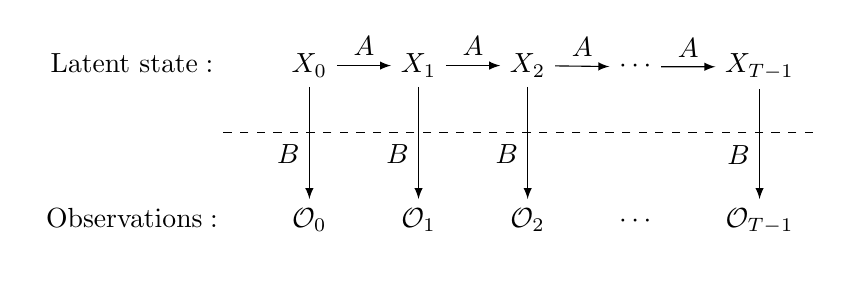
\begin{tikzpicture}
            \matrix[matrix of math nodes,column sep=2em,row sep=4em] (m) {
            \text{Latent state}: &
             X_0 & X_1 & X_2 & \cdots & X_{T-1}\\
            \text{Observations}: & 
             \mathcal{O}_0 & \mathcal{O}_1 & \mathcal{O}_2 & \cdots & \mathcal{O}_{T-1}\\
            };
            \foreach \X in {2,3,4,5}
            {\draw[-latex] (m-1-\X) -- (m-1-\the\numexpr\X+1) node[midway,above]{$A$};
            \ifnum\X=5
            \draw[-latex] (m-1-6) -- (m-2-6) node[pos=0.6,left]{$B$};
            \else
            \draw[-latex] (m-1-\X) -- (m-2-\X) node[pos=0.6,left]{$B$};
            \fi}
            \draw[dashed] ([yshift=1ex]m.east) -- ([yshift=1ex]m.east-|m-1-1.east);
            \end{tikzpicture}
        \caption{Hidden Markov Model}
        \label{fig:ch5:jointentropy}
    \end{figure}
       
    \section{Gilbert-Elliott Model}
    \begin{figure}[ht]
        \centering
        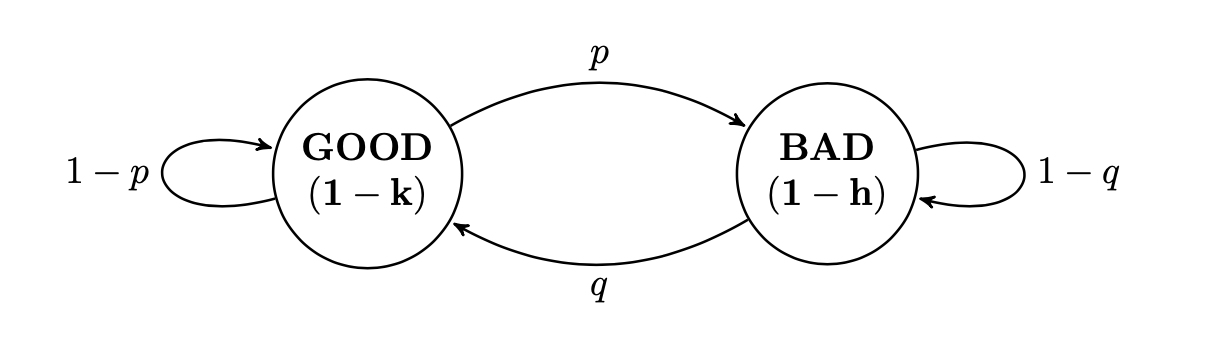
\includegraphics[scale=0.5]{figure1.png}
        \caption{Gilbert-Elliott Model}
        \label{fig:label}
    \end{figure}
\end{document}